\documentclass[tikz]{standalone}
\usetikzlibrary{intersections}
\begin{document}
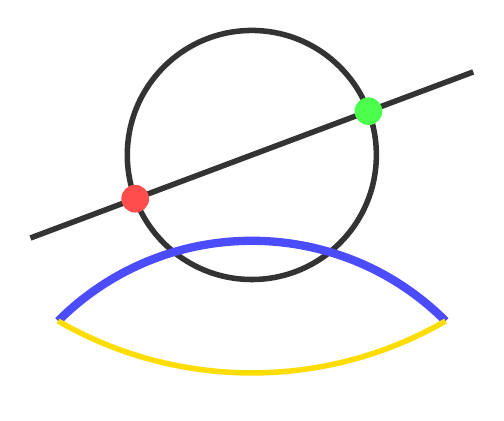
\begin{tikzpicture}[x=1pt,y=-1pt]
  \path[name path=rail] (30,110) -- (190,50);
  \path[name path=hoop] (110,80) circle (45);
  \path[name intersections={of=rail and hoop, by={x1, x2}}];
  \draw[color=black!80, line width=2] (30,110) -- (190,50);
  \draw[color=black!80, line width=2] (110,80) circle (45);
  \fill[red!70] (x1) circle (5);
  \fill[green!70] (x2) circle (5);
  \draw[blue!70, line width=3]
    (40,140) arc[start angle=225, end angle=315, radius=98.995];
  \draw[yellow!80!orange, line width=2]
    (40,140) arc[start angle=120, end angle=60, radius=140];
\end{tikzpicture}
\end{document}
